% Generated by Sphinx.
\def\sphinxdocclass{report}
\documentclass[A4paperpaper,11pt,english]{sphinxmanual}
\usepackage[utf8]{inputenc}
\DeclareUnicodeCharacter{00A0}{\nobreakspace}
\usepackage{cmap}
\usepackage[T1]{fontenc}
\usepackage{babel}
\usepackage{times}
\usepackage[Bjarne]{fncychap}
\usepackage{longtable}
\usepackage{sphinx}
\usepackage{multirow}

\usepackage{pdfpages}
\setcounter{tocdepth}{2}
% \makeatletter
% \def\cleardoublepage{
% \clearpage\if@twoside \ifodd\c@page\else
% \hbox{}
% \vspace*{\fill}
% \vspace{\fill}
% \thispagestyle{empty}
% \newpage
% \if@twocolumn\hbox{}\newpage\fi\fi\fi
% }
% \makeatother


\title{Actin Gels dynamics}
\date{March 13, 2014 at 18:32:57 CET}
\release{1.0}
\author{Matthias Bussonnier}
\newcommand{\sphinxlogo}{}
\renewcommand{\releasename}{Release}
\makeindex

\makeatletter
\def\PYG@reset{\let\PYG@it=\relax \let\PYG@bf=\relax%
    \let\PYG@ul=\relax \let\PYG@tc=\relax%
    \let\PYG@bc=\relax \let\PYG@ff=\relax}
\def\PYG@tok#1{\csname PYG@tok@#1\endcsname}
\def\PYG@toks#1+{\ifx\relax#1\empty\else%
    \PYG@tok{#1}\expandafter\PYG@toks\fi}
\def\PYG@do#1{\PYG@bc{\PYG@tc{\PYG@ul{%
    \PYG@it{\PYG@bf{\PYG@ff{#1}}}}}}}
\def\PYG#1#2{\PYG@reset\PYG@toks#1+\relax+\PYG@do{#2}}

\expandafter\def\csname PYG@tok@gd\endcsname{\def\PYG@tc##1{\textcolor[rgb]{0.63,0.00,0.00}{##1}}}
\expandafter\def\csname PYG@tok@gu\endcsname{\let\PYG@bf=\textbf\def\PYG@tc##1{\textcolor[rgb]{0.50,0.00,0.50}{##1}}}
\expandafter\def\csname PYG@tok@gt\endcsname{\def\PYG@tc##1{\textcolor[rgb]{0.00,0.27,0.87}{##1}}}
\expandafter\def\csname PYG@tok@gs\endcsname{\let\PYG@bf=\textbf}
\expandafter\def\csname PYG@tok@gr\endcsname{\def\PYG@tc##1{\textcolor[rgb]{1.00,0.00,0.00}{##1}}}
\expandafter\def\csname PYG@tok@cm\endcsname{\let\PYG@it=\textit\def\PYG@tc##1{\textcolor[rgb]{0.25,0.50,0.56}{##1}}}
\expandafter\def\csname PYG@tok@vg\endcsname{\def\PYG@tc##1{\textcolor[rgb]{0.73,0.38,0.84}{##1}}}
\expandafter\def\csname PYG@tok@m\endcsname{\def\PYG@tc##1{\textcolor[rgb]{0.13,0.50,0.31}{##1}}}
\expandafter\def\csname PYG@tok@mh\endcsname{\def\PYG@tc##1{\textcolor[rgb]{0.13,0.50,0.31}{##1}}}
\expandafter\def\csname PYG@tok@cs\endcsname{\def\PYG@tc##1{\textcolor[rgb]{0.25,0.50,0.56}{##1}}\def\PYG@bc##1{\setlength{\fboxsep}{0pt}\colorbox[rgb]{1.00,0.94,0.94}{\strut ##1}}}
\expandafter\def\csname PYG@tok@ge\endcsname{\let\PYG@it=\textit}
\expandafter\def\csname PYG@tok@vc\endcsname{\def\PYG@tc##1{\textcolor[rgb]{0.73,0.38,0.84}{##1}}}
\expandafter\def\csname PYG@tok@il\endcsname{\def\PYG@tc##1{\textcolor[rgb]{0.13,0.50,0.31}{##1}}}
\expandafter\def\csname PYG@tok@go\endcsname{\def\PYG@tc##1{\textcolor[rgb]{0.20,0.20,0.20}{##1}}}
\expandafter\def\csname PYG@tok@cp\endcsname{\def\PYG@tc##1{\textcolor[rgb]{0.00,0.44,0.13}{##1}}}
\expandafter\def\csname PYG@tok@gi\endcsname{\def\PYG@tc##1{\textcolor[rgb]{0.00,0.63,0.00}{##1}}}
\expandafter\def\csname PYG@tok@gh\endcsname{\let\PYG@bf=\textbf\def\PYG@tc##1{\textcolor[rgb]{0.00,0.00,0.50}{##1}}}
\expandafter\def\csname PYG@tok@ni\endcsname{\let\PYG@bf=\textbf\def\PYG@tc##1{\textcolor[rgb]{0.84,0.33,0.22}{##1}}}
\expandafter\def\csname PYG@tok@nl\endcsname{\let\PYG@bf=\textbf\def\PYG@tc##1{\textcolor[rgb]{0.00,0.13,0.44}{##1}}}
\expandafter\def\csname PYG@tok@nn\endcsname{\let\PYG@bf=\textbf\def\PYG@tc##1{\textcolor[rgb]{0.05,0.52,0.71}{##1}}}
\expandafter\def\csname PYG@tok@no\endcsname{\def\PYG@tc##1{\textcolor[rgb]{0.38,0.68,0.84}{##1}}}
\expandafter\def\csname PYG@tok@na\endcsname{\def\PYG@tc##1{\textcolor[rgb]{0.25,0.44,0.63}{##1}}}
\expandafter\def\csname PYG@tok@nb\endcsname{\def\PYG@tc##1{\textcolor[rgb]{0.00,0.44,0.13}{##1}}}
\expandafter\def\csname PYG@tok@nc\endcsname{\let\PYG@bf=\textbf\def\PYG@tc##1{\textcolor[rgb]{0.05,0.52,0.71}{##1}}}
\expandafter\def\csname PYG@tok@nd\endcsname{\let\PYG@bf=\textbf\def\PYG@tc##1{\textcolor[rgb]{0.33,0.33,0.33}{##1}}}
\expandafter\def\csname PYG@tok@ne\endcsname{\def\PYG@tc##1{\textcolor[rgb]{0.00,0.44,0.13}{##1}}}
\expandafter\def\csname PYG@tok@nf\endcsname{\def\PYG@tc##1{\textcolor[rgb]{0.02,0.16,0.49}{##1}}}
\expandafter\def\csname PYG@tok@si\endcsname{\let\PYG@it=\textit\def\PYG@tc##1{\textcolor[rgb]{0.44,0.63,0.82}{##1}}}
\expandafter\def\csname PYG@tok@s2\endcsname{\def\PYG@tc##1{\textcolor[rgb]{0.25,0.44,0.63}{##1}}}
\expandafter\def\csname PYG@tok@vi\endcsname{\def\PYG@tc##1{\textcolor[rgb]{0.73,0.38,0.84}{##1}}}
\expandafter\def\csname PYG@tok@nt\endcsname{\let\PYG@bf=\textbf\def\PYG@tc##1{\textcolor[rgb]{0.02,0.16,0.45}{##1}}}
\expandafter\def\csname PYG@tok@nv\endcsname{\def\PYG@tc##1{\textcolor[rgb]{0.73,0.38,0.84}{##1}}}
\expandafter\def\csname PYG@tok@s1\endcsname{\def\PYG@tc##1{\textcolor[rgb]{0.25,0.44,0.63}{##1}}}
\expandafter\def\csname PYG@tok@gp\endcsname{\let\PYG@bf=\textbf\def\PYG@tc##1{\textcolor[rgb]{0.78,0.36,0.04}{##1}}}
\expandafter\def\csname PYG@tok@sh\endcsname{\def\PYG@tc##1{\textcolor[rgb]{0.25,0.44,0.63}{##1}}}
\expandafter\def\csname PYG@tok@ow\endcsname{\let\PYG@bf=\textbf\def\PYG@tc##1{\textcolor[rgb]{0.00,0.44,0.13}{##1}}}
\expandafter\def\csname PYG@tok@sx\endcsname{\def\PYG@tc##1{\textcolor[rgb]{0.78,0.36,0.04}{##1}}}
\expandafter\def\csname PYG@tok@bp\endcsname{\def\PYG@tc##1{\textcolor[rgb]{0.00,0.44,0.13}{##1}}}
\expandafter\def\csname PYG@tok@c1\endcsname{\let\PYG@it=\textit\def\PYG@tc##1{\textcolor[rgb]{0.25,0.50,0.56}{##1}}}
\expandafter\def\csname PYG@tok@kc\endcsname{\let\PYG@bf=\textbf\def\PYG@tc##1{\textcolor[rgb]{0.00,0.44,0.13}{##1}}}
\expandafter\def\csname PYG@tok@c\endcsname{\let\PYG@it=\textit\def\PYG@tc##1{\textcolor[rgb]{0.25,0.50,0.56}{##1}}}
\expandafter\def\csname PYG@tok@mf\endcsname{\def\PYG@tc##1{\textcolor[rgb]{0.13,0.50,0.31}{##1}}}
\expandafter\def\csname PYG@tok@err\endcsname{\def\PYG@bc##1{\setlength{\fboxsep}{0pt}\fcolorbox[rgb]{1.00,0.00,0.00}{1,1,1}{\strut ##1}}}
\expandafter\def\csname PYG@tok@kd\endcsname{\let\PYG@bf=\textbf\def\PYG@tc##1{\textcolor[rgb]{0.00,0.44,0.13}{##1}}}
\expandafter\def\csname PYG@tok@ss\endcsname{\def\PYG@tc##1{\textcolor[rgb]{0.32,0.47,0.09}{##1}}}
\expandafter\def\csname PYG@tok@sr\endcsname{\def\PYG@tc##1{\textcolor[rgb]{0.14,0.33,0.53}{##1}}}
\expandafter\def\csname PYG@tok@mo\endcsname{\def\PYG@tc##1{\textcolor[rgb]{0.13,0.50,0.31}{##1}}}
\expandafter\def\csname PYG@tok@mi\endcsname{\def\PYG@tc##1{\textcolor[rgb]{0.13,0.50,0.31}{##1}}}
\expandafter\def\csname PYG@tok@kn\endcsname{\let\PYG@bf=\textbf\def\PYG@tc##1{\textcolor[rgb]{0.00,0.44,0.13}{##1}}}
\expandafter\def\csname PYG@tok@o\endcsname{\def\PYG@tc##1{\textcolor[rgb]{0.40,0.40,0.40}{##1}}}
\expandafter\def\csname PYG@tok@kr\endcsname{\let\PYG@bf=\textbf\def\PYG@tc##1{\textcolor[rgb]{0.00,0.44,0.13}{##1}}}
\expandafter\def\csname PYG@tok@s\endcsname{\def\PYG@tc##1{\textcolor[rgb]{0.25,0.44,0.63}{##1}}}
\expandafter\def\csname PYG@tok@kp\endcsname{\def\PYG@tc##1{\textcolor[rgb]{0.00,0.44,0.13}{##1}}}
\expandafter\def\csname PYG@tok@w\endcsname{\def\PYG@tc##1{\textcolor[rgb]{0.73,0.73,0.73}{##1}}}
\expandafter\def\csname PYG@tok@kt\endcsname{\def\PYG@tc##1{\textcolor[rgb]{0.56,0.13,0.00}{##1}}}
\expandafter\def\csname PYG@tok@sc\endcsname{\def\PYG@tc##1{\textcolor[rgb]{0.25,0.44,0.63}{##1}}}
\expandafter\def\csname PYG@tok@sb\endcsname{\def\PYG@tc##1{\textcolor[rgb]{0.25,0.44,0.63}{##1}}}
\expandafter\def\csname PYG@tok@k\endcsname{\let\PYG@bf=\textbf\def\PYG@tc##1{\textcolor[rgb]{0.00,0.44,0.13}{##1}}}
\expandafter\def\csname PYG@tok@se\endcsname{\let\PYG@bf=\textbf\def\PYG@tc##1{\textcolor[rgb]{0.25,0.44,0.63}{##1}}}
\expandafter\def\csname PYG@tok@sd\endcsname{\let\PYG@it=\textit\def\PYG@tc##1{\textcolor[rgb]{0.25,0.44,0.63}{##1}}}

\def\PYGZbs{\char`\\}
\def\PYGZus{\char`\_}
\def\PYGZob{\char`\{}
\def\PYGZcb{\char`\}}
\def\PYGZca{\char`\^}
\def\PYGZam{\char`\&}
\def\PYGZlt{\char`\<}
\def\PYGZgt{\char`\>}
\def\PYGZsh{\char`\#}
\def\PYGZpc{\char`\%}
\def\PYGZdl{\char`\$}
\def\PYGZhy{\char`\-}
\def\PYGZsq{\char`\'}
\def\PYGZdq{\char`\"}
\def\PYGZti{\char`\~}
% for compatibility with earlier versions
\def\PYGZat{@}
\def\PYGZlb{[}
\def\PYGZrb{]}
\makeatother

\begin{document}

\maketitle

% \\pagestyle{frontmatter}
% \\chapter*{Abstract}
% \\thispagestyle{frontmatter}
% %s
% \\chapter*{Foreword}
% \\thispagestyle{frontmatter}
% %s
% \\chapter*{Acknowledgements}
% \\thispagestyle{frontmatter}
% --s
\tableofcontents
% \\cleardoublepage
% \\pagestyle{frontmatter}
% \\addtocontents{toc}{\\protect\\thispagestyle{frontmatter}}
% \\listoffigures
% \\addtocontents{lof}{\\protect\\thispagestyle{frontmatter}}
% \\listoftables
% \\addtocontents{lot}{\\protect\\thispagestyle{frontmatter}}
\cleardoublepage
\pagestyle{normal}
\pagenumbering{arabic}
 
\phantomsection\label{index-latex::doc}



\chapter{Background}
\label{parts/part1::doc}\label{parts/part1:background}\label{parts/part1:contents}
\begin{notice}{note}{Todo}
\begin{itemize}
\item {} 
Even in mitosis for big cell, actin is needed to assemble chromosoms {\hyperref[bibitem:lenart2005]{{[}Lenart, Bacher, Daigle,  et al.  2005{]}}}

\item {} 
Rapid change in actin structure {\hyperref[bibitem:vasilev2012]{{[}Vasilev, Chun, Gragnaniello,  et al.  2012{]}}}, timing is also important (exposition to inomycine disrupt cortex functionality)

\item {} 
F-actin network cabable of supporting mechanical load {\hyperref[bibitem:feric2013]{{[}Feric, Brangwynne,  2013{]}}}

\item {} 
Presence of f-Actin meshwork meshsize \textasciitilde{}0.5µm {\hyperref[bibitem:feric2013]{{[}Feric, Brangwynne,  2013{]}}}

\item {} 
This actin network can wistant repetitive compression {\hyperref[bibitem:feric2013]{{[}Feric, Brangwynne,  2013{]}}}

\item {} 
F actin network might be linked to the lamin (a kind of IF) cortex around the nucleus {\hyperref[bibitem:feric2013]{{[}Feric, Brangwynne,  2013{]}}}

\item {} 
Such a network woudl only need to sutain a pressure on the order od 0.01 PA {\hyperref[bibitem:feric2013]{{[}Feric, Brangwynne,  2013{]}}},
and is essential to fight agains gravity

\end{itemize}
\end{notice}


\section{Introduction}
\label{parts/part1:introduction}
Cells are the basic component of living organism, understanding their
individual behavior and the way they function is a key step into understanding
how they interact with their environment and other organism. One of the key
component to most of organism is Actin, a protein which is highly conserved
across the species and play a important role in cell mechanics, from cell
migration to cell differentiation and division. It plays also a non negligible
in most mechanical properties of the cell and how it interacts with its
environment. In particular actin is the main component of the actin cortex :
the part of the cell cytoskeleton below the plasma membrane mostly responsible
for cell mechanical properties. The properties of this actin cortex is drive by
the mechanics of the properties of its main component : a dynamic actin
network. Understanding this actin network is hence a key piece to learn how
the actin cortex behave.

The properties of an actin network highly depend on it's structure. The
structure itself depends on many parameters that influence how the network is
formed. Network structure and formation can be not only influence by its
physical and chemical environments but also by the variation of this
parameters with time and space.

Cells are complex systems that adapt their shape, mechanical properties and
biochemical conditions permanently. The spacial repartition of theses
properties is also variable as the cell regulate the concentration of proteins
all across its body. To well study the effect of each components independently,
it is crucial to study actin network in a controlled environment.

Biomimetic systems allow to respond to most of these concern, they provide a
well controlled environment where biochemical condition can be well controlled
both in space and time. Theses systems keep their biological relevance, as they
can mimic \emph{in vivo} phenomenon. Biomimetic systems are also well adapted to the
tools available and the approach from a physics point of view. The optical trap
will allow us to study local mechanical properties of actin  network  with a
high time resolution which could allow to get insight into the variation of
theses properties as a function of time.

During my PhD, my work has mainly be to study the mechanics of branched actin
network polymerizing on optically trapped polystyrene beads. Such network was
studied before {\hyperref[bibitem:kawska2012]{{[}Kawska, Carvalho, Manzi,  et al.  2012{]}}}  but have suspected to be highly inhomogeneous,
the use of optical trap allowed to probe mechanics of part of the network
unaccessible before.
\begin{itemize}
\item {} 
time resolution

\item {} 
network dynamics

\item {} 
Move to liposome,

\item {} 
study in OOCyte :

\item {} 
Basically from purely biiomimetic to real cells

\end{itemize}


\section{Living Cells}
\label{parts/part1:living-cells}
\begin{notice}{note}{Todo}
\end{notice}

\begin{notice}{note}{Todo}

We can see in plants that actin, also known as microfilament
{\hyperref[bibitem:iwabuchi2010]{{[}Iwabuchi, Takagi,  2010{]}}} is used to move nucleus away from
\end{notice}

Cells are the smallest living component which are present from unicellular
plants to multicellular animals. Thus, cells should cover a huge range of
behavior going from extremely specific on multicellular organism, to all the
function that are needed to survive and reproduce for bacterial colony.
Multicellular organism will grow specialized cell from neurone to osteoblast
going through germinal or muscle cells. In the other hand, unicellular
organisms are made of cell that are responsible for all the function of the
organism, from motility to reproduction, passing through absorption of
nutriment to replication of the cell.

Cell are hence able to adapt to their environment as a function of time, and
also have function and behavior that depends on time, and a small change of
timing and/or biochemical conditions can highly injure the development of an
organism {\hyperref[bibitem:lenart2005]{{[}Lenart, Bacher, Daigle,  et al.  2005{]}}}, it has also been observe that the mechanical
properties of substrate can govern the differentiation of cell
{\hyperref[bibitem:engler2006]{{[}Engler, Sen, Sweeney, Discher,  2006{]}}} .

Nonetheless, even with all theses different behavior and phenotype, the cells
all have a common structure. They are constituted by a membrane which is
responsible form separating the cytoplasm from the outside of the cell. The
cytoplasm contains organelles, genetic material, and number of proteins that
the cell use to accomplish its functions. Cells are of course not completely
isolated, and have numbers of mechanism to exchange and communicate with the
outside. Communication with the outside are either chemical or mechanics.  To
sens their mechanical environment, cell use adhesion complexes to attach to the
medium, and integrins as trans-membrane protein will transfer the force to the
cell cytoskeleton situated inside the cell.
\begin{figure}[htbp]
\centering
\capstart

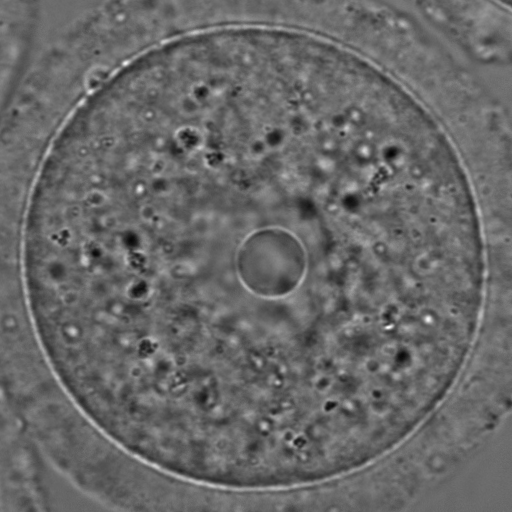
\includegraphics[width=0.700\linewidth]{oocyte-wild-type.png}
\caption{Bright field image of a mouse oocyte before meiosis. Cell diameter is
of 80 µm. The nucleus can be clearly seen at the center of the
cell. Image Credit to Maria Almonacid from Collège de France.}\label{parts/part1:oocytewt}\end{figure}

This structure, which is situated just below the cell membrane, is named the
actin cortex,


\subsection{The Cell Cytoskeleton}
\label{parts/part1:the-cell-cytoskeleton}
The cytoskeleton, literally skeleton of the cell, is the structure which give
it shape to a cell.  As for other multicellular animals that possesses
skeleton, its shape is often a hint on how a organism move. As feet, fins and
wigs are characteristics that will tell you whether a animal does more
preferably prefer land, see or air, the cytoskeleton is will tell you many
things a bout a cell.

In the other hand, unlike (exo)-Skeleton of animals which is ridged and
unchanging, the cytoskeleton of cell is a  highly dynamic structure that keep
remodeling itself on a short time scale compared to the speed at which a cell
move. That's through this dynamics that the cytoskeleton can achieve its
functions.  As mammals skeletons are necessary to transmit force from one part
of the body to another, the cell cytoskeleton is responsible to not only
transmit the force the cell is exerting, but also to generate theses force.
Thats through its cytoskeleton that a cell can be connected to its environment,
both mechanically and biochemically.

\begin{notice}{note}{Todo}

trouver des ref pour ci dessous
\end{notice}

The cytoskeleton is mainly composed of three type of filaments.  The
microtubules, intermediate filament and actin filament, also known as
microfilament.


\subsubsection{Microtubules}
\label{parts/part1:microtubules}
Microtubules are the wider with a diameter of 20nm and {[}un article où on voit le diameter{]} the stiffer of the three kinds of filament with a persistence
length in the order of millimeter, which is much longer than the size of the
usual cell. Microtubules are extensively studied {[}cite some reviews ...{]}.
Microtubules form polar (oriented) filament that can be walked on by molecular
motors that can be decomposed in two families – kinesins  and dyneins –
depending on the end toward which the motor preferably walk. Microtubules are
mostly known for their action during the cells mitosis where they will form
majority of the mitotic spindle that drive the segregation of the chromosomes
in two groups, each group ending in one of the daughter cells.

We will not be interested directly into the effect and behavior of microtubules
in this manuscript.


\subsubsection{Intermediate filaments}
\label{parts/part1:intermediate-filaments}
Intermediate filaments are of medium diameter in the order of around 10nm, in
between actin and microtubules filament, hence their name.  Unlike microtubules
and actin filament, intermediate filaments are composed by several sub-families
of proteins and are non-polar.


\subsubsection{Actin}
\label{parts/part1:actin}
Actin, is the third component of the cytoskeleton, the one we will focus most
of our effort. Actin can forms actin filament, the thinest of the three kind
that form the cytoskeleton. Actin is produced in the cell as a globular protein
of \textasciitilde{}40 kDa that once associated with ATP or ADP polymerise into helicoidal
filament with a diameter between 7 and 9nm. The formed actin filament are
polar, which both extremity respectively called the plus (\emph{+}) or
barbed end, and the minus (\emph{-}) or pointed end. The polarity of the actin
filament is of importance as this give rise to a proved direction for most
processes that can happen on the filament.

The actin protein is highly conserved across species, and is know to directly
interact with hundreds of proteins {\hyperref[bibitem:dosremedios2003]{{[}dRemedios, Chhabra, Kekic,  et al.  2003{]}}}. As hint before it can in particular bind to ATP, that can hydrolyse into,


\paragraph{Dynamic of actin polymerisation}
\label{parts/part1:dynamic-of-actin-polymerisation}
The assembly mechanism that allow to go from singles monomers of actin (also
refer to as G-actin in solution) to actin filament (also refer as F-actin)
need to be well understood to explain the different structure of network actin
filament can give once put in presence of other proteins.

The polymerisation of ATP/ADP actin monomer to form an actin filament need to go
through the step of forming a actin proto-filament which is constituted of at
least 3 actin monomers. This will most of the time be the kinetically limiting
step. Once proto-filaments are present in solution, single monomers can be
freely added or removed on both end of the filament.

We now need to distinguish between the dynamic of adding or removing on both
ends of the filament. Indeed it has been show that the association and
dissociation rate are differing between the pointed (-) and barbed (+) end.
More particularly, the association rate at the barbed rate is higher that on
the pointed end, and same goes for the dissociation rate which has a bigger
constant on the minus end of actin filament. This lead to in imbalance of actin
(de)-polymerisation on both ends, which leads to actin filament preferably
growing on the barbed end and preferably shrinking from the pointed end.

The equations that drive the polymerisation can thus be written as follow
\begin{gather}
\begin{split}\frac{dC_b}{dt} &= k_{+,b}.[monomers] - k_{-,b} \\
\frac{dC_p}{dt} &= k_{+,p}.[monomers] - k_{-,p} \\\end{split}\notag
\end{gather}
Where \emph{b} and \emph{p} designate respectively the barbed and pointed end, and
\(k_+\) and \(k_-\) are the polymerisation and depolymerisation rate.
The concentration in barbed and pointed end denoted by \(C_\_\). By
assuming that the number of pointed end is equal to the number of barbed end,
one can derive the steady state which give rise to the critical monomer
concentration below which a actin filament cannot grow: \([monomers]_c\).

The rate constant of elongation of actin have been determined to also depend of
whether the monomer was bound to ADP or ATP {\hyperref[bibitem:pollard1986]{{[}Pollard,  1986{]}}}. We should now
consider the fact that ATP-bound actin will hydrolyse to ADP-Pi then release
the inorganic phosphate, and thus with a rate that also depend on whether the
monomer is part of a filament or in solution.

It should be noted that the in stationary state the length of each actin
filaments statistically constant because the speed of polymerisation on the
barbed end is compensated by the depolymerisation on the pointed end. The
filament is hence in a threadmilling state. If we follow a single actin monomer
bound to an ATP molecule, it will be incorporated at the \emph{+} end of the
filament and progressively move toward the minus end, eventually hydrolysing
it's ATP into ADP before detecting from the filament on the pointed end.

\begin{notice}{note}{Todo}
\begin{itemize}
\item {} 
cf fletcher 2010 review {\hyperref[bibitem:fletcher2010]{{[}Fletcher, Mullins,  2010{]}}} the cytoskeleton as 3 main
functions :
\begin{itemize}
\item {} 
organize cell in space

\item {} 
connect cell to external environment (biochemical and mechanical)

\item {} 
generate and coordinate force to allow cell to change shape.

\item {} 
some things on temporal and spacial effect of structures like ``bud scar''

\item {} 
schema of branched Arp2/3 actin factor

\end{itemize}

\item {} 
Loading history determines the velocity of actin-network growth
{\hyperref[bibitem:parekh2005]{{[}Parekh, Chaudhuri, Theriot, Fletcher,  2005{]}}} hence network can record history, single filament
cannot.

\end{itemize}
\end{notice}


\paragraph{Proteins influencing actin polymerisation}
\label{parts/part1:proteins-influencing-actin-polymerisation}
Despite the already complex process that is actin polymerisation and the
numbers of parameter that we have already introduce, the formation of an actin
network is a even more complex process that involve many other components.
Especially, actin monomers and filament can interact with a high number of
proteins that will effect previously established dynamics.  We will present
some categories of such preoteins.


\subparagraph{Polymerase family}
\label{parts/part1:polymerase-family}
The polymerase family as their name indicate will directly have effect on the
polymerisation of actin. In the right condition, polymerase will increase the
\(k_+\) at one end of the actin filament for the same concentration of
actin monomers. This can lead to an average longer filament length.

\emph{Formins} Are one of those polymerase proteins that will
increase the polymerisation rate at the barbed end. It has the particularity of
being processive, meeting that it will stay bound to the barbed and while
catalysing the addition on new monomers.


\subparagraph{Crosslinkers}
\label{parts/part1:crosslinkers}

\subparagraph{Stabilising proteins}
\label{parts/part1:stabilising-proteins}

\subparagraph{Capping Protein}
\label{parts/part1:capping-protein}
\begin{notice}{note}{Todo}
\begin{itemize}
\item {} 
more than 150 protein have been found to bind with actin.

\item {} 
Wave complex,
\begin{itemize}
\item {} 
Wasp, N-Wasp ( need to cite \emph{Machesky1999} )

\end{itemize}

\item {} 
Not composed only by actin

Should cite \emph{Pollard2003}
\begin{itemize}
\item {} 
Some network need actin, some other do not. (Fletcher review 2010)

\item {} 
NPF

\item {} 
Polymerase, (depolymerase severing),

\item {} 
crosslinker,
\begin{itemize}
\item {} 
// like fascine
\begin{itemize}
\item {} 
rotate like alpha-acitinnin

\item {} 
effect of cross linking distance {[}Morse20..{]}

\end{itemize}

\end{itemize}

\item {} 
stabilizing

\item {} 
Moleular motors.

\item {} 
interphase, cellule prepare for division

\item {} 
Mitosis : ``DNA Segregating''

\item {} 
need to describe actin,
\begin{itemize}
\item {} 
depending on the length scale semi-flexible polymers.

\end{itemize}

\item {} 
polymerisation barbed end pointed end, (directed)
\begin{itemize}
\item {} 
form microfilement

\end{itemize}

\item {} 
cytoskeleton is dynamic

\item {} 
formed under the plasme membrane

\item {} 
ratchet nechanisme

\item {} 
use of Arp2/3 to branch

\item {} 
capping, protein,  formin (OOcyte)

\item {} 
myosin, run on actin to barbed end/ processive/not processive.
\begin{itemize}
\item {} 
stress fibres

\end{itemize}

\item {} 
troppomyosine

\end{itemize}

\end{itemize}

All the living kingdom is characterised by the fact that organism can reproduce,
\end{notice}

And


\subsection{Cell Organelle}
\label{parts/part1:cell-organelle}\begin{itemize}
\item {} 
Mitoncondria, ER (made to produce proteins), also serve in lacust

\item {} 
nucleus en eucariotes cells, contains the chromosomes.

\item {} 
Nucleus get moved by actin filement to the periclinal/anticlinal wall,

\item {} 
centromere centriole,

\item {} 
Organelles are supported by

\end{itemize}


\section{The Role Of Actin Cytoskeletton}
\label{parts/part1:the-role-of-actin-cytoskeletton}

\subsection{Cell Motility}
\label{parts/part1:cell-motility}

\subsection{The actin cortex}
\label{parts/part1:the-actin-cortex}

\subsection{Organelle Positioning (actin cloud)}
\label{parts/part1:organelle-positioning-actin-cloud}

\subsection{Nuclear positionning during miosis}
\label{parts/part1:nuclear-positionning-during-miosis}

\section{In vitro reconstituted actin networks}
\label{parts/part1:in-vitro-reconstituted-actin-networks}

\section{Actin networks as viscoelastic material}
\label{parts/part1:actin-networks-as-viscoelastic-material}

\section{Active and Passive microrheologie}
\label{parts/part1:active-and-passive-microrheologie}

\section{Optical tweezer}
\label{parts/part1:optical-tweezer}

\section{Membrane Physics}
\label{parts/part1:membrane-physics}

\section{Myosis (to move away)}
\label{parts/part1:myosis-to-move-away}
\begin{notice}{note}{Todo}
\begin{itemize}
\item {} 
Asymetric division of oocyte,

\item {} 
from diploid, to haploid,
- spindle usually in mmithosis pulled by microtubule

\end{itemize}
\end{notice}


\chapter{Materials and methods}
\label{parts/part2::doc}\label{parts/part2:materials-and-methods}

\section{Actin}
\label{parts/part2:actin}

\section{Profiline}
\label{parts/part2:profiline}

\section{Arp2/3}
\label{parts/part2:arp2-3}
{\hyperref[bibitem:goley2006]{{[}Goley, Welch,  2006{]}}}


\section{Bead Motility}
\label{parts/part2:bead-motility}

\section{3D fitting}
\label{parts/part2:d-fitting}

\section{?? ?? ??}
\label{parts/part2:id2}

\chapter{Results}
\label{parts/part3::doc}\label{parts/part3:results}

\section{Actin Cloud}
\label{parts/part3:actin-cloud}

\section{Doublets}
\label{parts/part3:doublets}

\section{Oocytes}
\label{parts/part3:oocytes}

\chapter{Discussion}
\label{parts/part4:discussion}\label{parts/part4::doc}

\chapter{Optical Trap Setup}
\label{parts/physicalparameters:physicalparameters}\label{parts/physicalparameters::doc}\label{parts/physicalparameters:optical-trap-setup}

\section{Preface}
\label{parts/physicalparameters:preface}
In order to manipulate the polystyrene beads that are used in the different
experiments, I worked on a already build setup with time shared optical trap

To investigate the effect of different actin network on mechanics of cell
behavior, Sykes team of curie institute is specialized in using biomimetics
sytems. In particular, polystyrene actin bead covered with nucleator of actin
polymerisation have been developped as a biomimetic system of listeria
monocytogen. It is such a system that I have studied.

By growing actin network in controlled condition I was able to reproductibly
determine mechanical properties.


\section{Choice of experimental tools}
\label{parts/physicalparameters:choice-of-experimental-tools}
The choice of experimental tools, and experimental conditions is important to
determine in the range of properties and parameters you can access to.
Previous and ongoing studies at the time were focused on the properties of dense
gel in comets tails, as well as the one around the polystyrene beads, as well as the one on the surface before symetry breaking.


\chapter{Liposome doublets}
\label{parts/physicalparameters:liposome-doublets}
In this chapter we study the comportment of what we will refer as ``Doublets'';
an biomimetic system that allow us to study quantitatively the tension on a
membrane covered with a actin shell mimicking the cells actin cortex. Even if
such a system has already been studied, we believe that the new technique we
develop can allow the non-invasive measure of variation of tension on liposome.
\begin{figure}[htbp]
\centering
\capstart

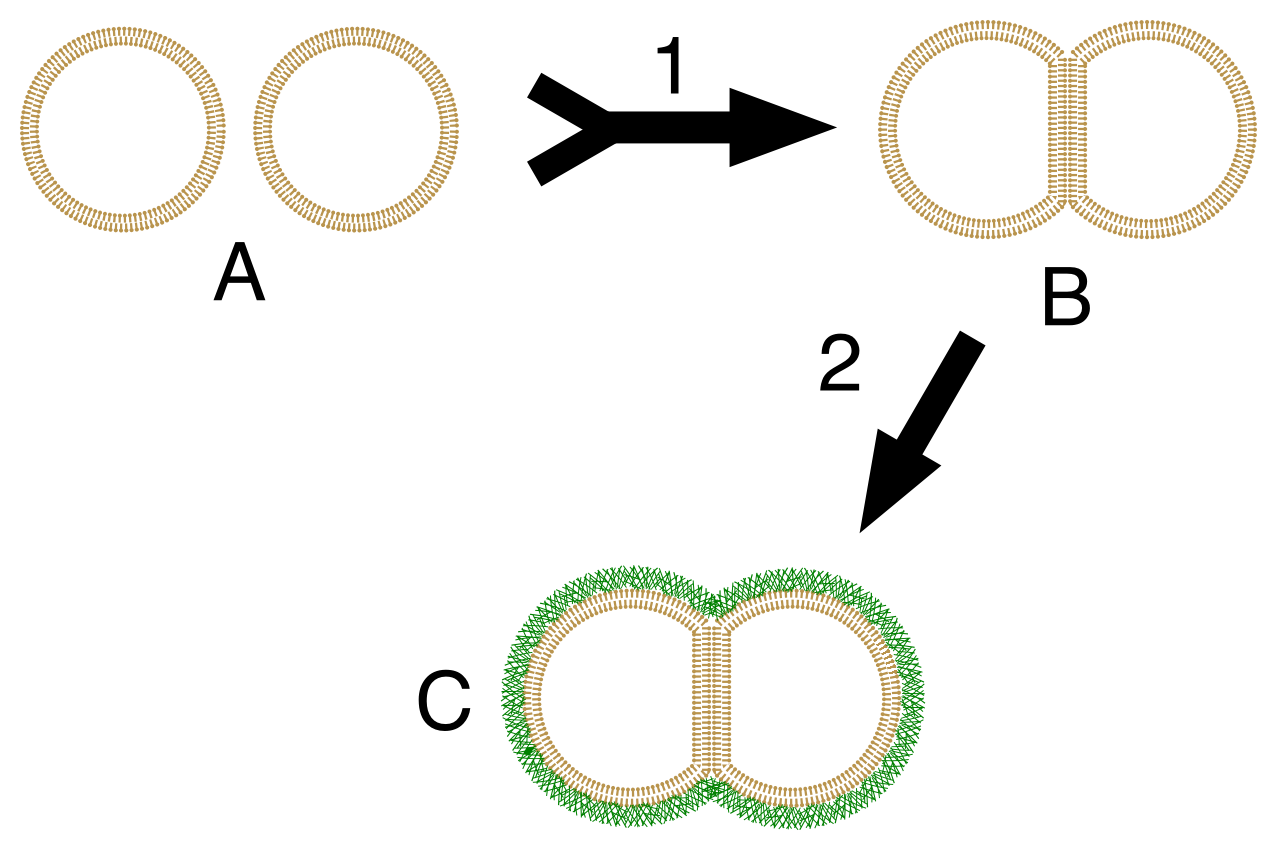
\includegraphics{doublets-schema.png}
\caption{Single liposome can formxe a doublets with a single double double layer
separating them, adhere with a double bi-layer, or cover with atin.  Bare
doublets can then get covered with actin and actin covered liposome can
adhere together. The two kinds of doublets can be differentiated by using
fluorescently labeled acctin.}\label{parts/physicalparameters:figdoubletsschema}\end{figure}

Starting with a liposome solution containing
biotinilated actin filament and streptavidine doublet will naturally
occurs. Liposomes will either adhere before or after being covered with
actin filament. In the rest of this chapter we are interested in studying
only the case where both liposome adhere before being in coverd with actin.
To increase the ratio of both kinds of doublet, the solution of liposome is
gently centrifuged before adding the F-actin into the mix. As experiments
were done using fluorescently labeled actin, the discrimination between the
two kinds of doublets was easily done looking at the fluorescent intensity
on the interface between the two doublets. Only doublet where no signal on
the interface was visible were analysed.


\section{Relating Doublets to Living cell}
\label{parts/physicalparameters:relating-doublets-to-living-cell}
Determining contact angle in cell is the often use methods to determine effective tension of membrane linked to cythoskeleton. :cite:Leon Maitre:


\section{Doublets geometric parameter}
\label{parts/physicalparameters:doublets-geometric-parameter}
Using biomimetic system allow to more control over a system and decrease the
number of parameter one have to study to better understand there influence.
Unlike cell that are active and constantly shape changing, liposome have a
shape that follow a smaller number of physical law. This translate in the right
condition to liposome taking a spherical form. Knowing this information we
derived a methods to determine the contact angle between liposome in a less
experimentor biased way.

In this section we will show that the geometrical parameters of a doublet can
be modeled by the combinaison of two intersecting sphere, simulate the
fluorescent image that such a doublet would generate  and show that we can
optimise the parameters of the model to reflect the exerimental data thus
determining the actual geometrical parameter of the doublets in an experimentor
independant mater by also automatising the system.

In the following par we will restrain ourselves to example in a two dimensional
space for easier visualisation and work in pixel for convenience


\subsection{Finding a single liposome}
\label{parts/physicalparameters:finding-a-single-liposome}
Experimentally liposomes are observed using fluorescently labeled component, in
particular we used a GFP labeled actin and streptavidine that will be imaged
using a inverted microscope. In the observation plane, the liposome formed
using fluorescently labeled streptavine will form a bright ringi of given
thickness.  When imaging the actin shell, assuming the actinshell is of
homogeneous thickness around the liposome will also manifest as a fluorecent ring.

In the case where the membrane is marked, the radius of liposome will be the median radius of the ring.

In the case of actin shell, when the thickness of the actin shell is bigger compared the resolution limit of our method, then the liposome radius should be taken as the inner raius of the ring
\begin{figure}[htbp]
\centering
\capstart

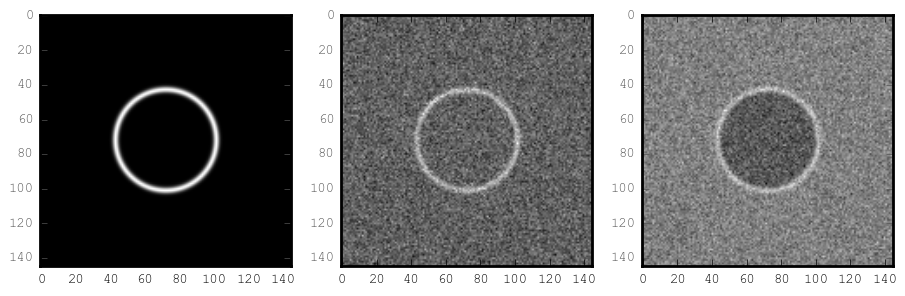
\includegraphics{modl-2d-doublet.png}
\caption{Left : A simulation of liposome fluorescent of an uniform shell or
membrane.
Middle: Same Image Adding gaussian noise to simulate a plane from
a confocal Z-stack.
Right: Fluorescently labelled Liposome in fluorescent External Buffer
and non fluorescent medium.}\end{figure}
\begin{figure}[htbp]
\centering

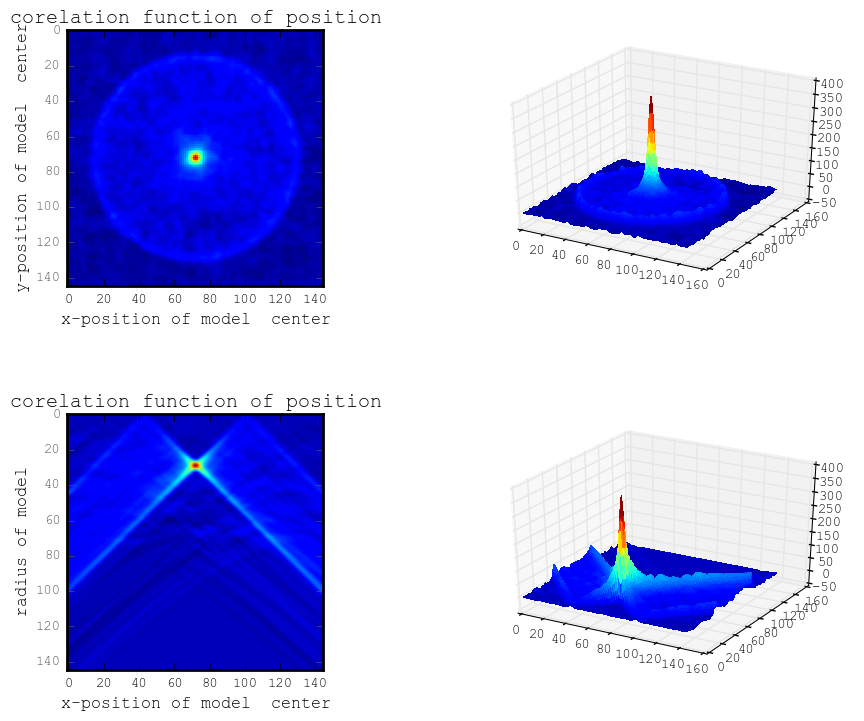
\includegraphics{corrfun-noise-.png}
\end{figure}
\begin{itemize}
\item {} 
\emph{search}

\end{itemize}

\begin{notice}{note}{Note:}
You can Download the latest pdf version of this
document.
\end{notice}


\chapter{References}
\label{index-latex:references}


\begin{thebibliography}{Parekh, Chaudhuri, Theriot, Fletcher,  2005}
\bibitem[dRemedios, Chhabra, Kekic,  et al.  2003]{dRemedios, Chhabra, Kekic,  et al.  2003}{\phantomsection\label{bibitem:dosremedios2003} 
C G dos Remedios, D Chhabra, M Kekic, I V Dedova, M Tsubakihara, D A Berry, and N J Nosworthy. Actin binding proteins: regulation of cytoskeletal microfilaments.. \emph{Physiological reviews}, 83(2):433–73, April 2003. \href{http://www.ncbi.nlm.nih.gov/pubmed/12663865}{URL: http://www.ncbi.nlm.nih.gov/pubmed/12663865}, \href{http://dx.doi.org/10.1152/physrev.00026.2002}{doi:10.1152/physrev.00026.2002}.
}
\bibitem[Engler, Sen, Sweeney, Discher,  2006]{Engler, Sen, Sweeney, Discher,  2006}{\phantomsection\label{bibitem:engler2006} 
Adam J. Engler, Shamik Sen, H. Lee Sweeney, and Dennis E. Discher. Matrix elasticity directs stem cell lineage specification.. \emph{Cell}, 126(4):677–89, August 2006. \href{http://www.ncbi.nlm.nih.gov/pubmed/16923388}{URL: http://www.ncbi.nlm.nih.gov/pubmed/16923388}, \href{http://dx.doi.org/10.1016/j.cell.2006.06.044}{doi:10.1016/j.cell.2006.06.044}.
}
\bibitem[Feric, Brangwynne,  2013]{Feric, Brangwynne,  2013}{\phantomsection\label{bibitem:feric2013} 
Marina Feric and Clifford P Brangwynne. A nuclear F-actin scaffold stabilizes ribonucleoprotein droplets against gravity in large cells. \emph{Nature Cell Biology}, 15:1253–1259, 2013. \href{http://dx.doi.org/10.1038/ncb2830}{URL: http://dx.doi.org/10.1038/ncb2830}, \href{http://dx.doi.org/10.1038/ncb2830}{doi:10.1038/ncb2830}.
}
\bibitem[Fletcher, Mullins,  2010]{Fletcher, Mullins,  2010}{\phantomsection\label{bibitem:fletcher2010} 
Daniel A Fletcher and R Dyche Mullins. Cell mechanics and the cytoskeleton.. \emph{Nature}, 463(7280):485–92, January 2010. \href{http://dx.doi.org/10.1038/nature08908 http://www.pubmedcentral.nih.gov/articlerender.fcgi?artid=2851742\&tool=pmcentrez\&rendertype=abstract}{URL: http://dx.doi.org/10.1038/nature08908 http://www.pubmedcentral.nih.gov/articlerender.fcgi?artid=2851742\&tool=pmcentrez\&rendertype=abstract}, \href{http://dx.doi.org/10.1038/nature08908}{doi:10.1038/nature08908}.
}
\bibitem[Goley, Welch,  2006]{Goley, Welch,  2006}{\phantomsection\label{bibitem:goley2006} 
Erin D Goley and Matthew D Welch. The ARP2/3 complex: an actin nucleator comes of age.. \emph{Nature reviews. Molecular cell biology}, 7(10):713–26, October 2006. \href{http://dx.doi.org/10.1038/nrm2026}{URL: http://dx.doi.org/10.1038/nrm2026}, \href{http://dx.doi.org/10.1038/nrm2026}{doi:10.1038/nrm2026}.
}
\bibitem[Iwabuchi, Takagi,  2010]{Iwabuchi, Takagi,  2010}{\phantomsection\label{bibitem:iwabuchi2010} 
Kosei Iwabuchi and Shingo Takagi. Actin-based mechanisms for light-dependent intracellular positioning of nuclei and chloroplasts in Arabidopsis.. \emph{Plant signaling \& behavior}, 5(8):1010–3, August 2010. \href{http://www.plantphysiol.org/content/152/3/1309}{URL: http://www.plantphysiol.org/content/152/3/1309}, \href{http://dx.doi.org/10.1104/pp.109.149526}{doi:10.1104/pp.109.149526}.
}
\bibitem[Kawska, Carvalho, Manzi,  et al.  2012]{Kawska, Carvalho, Manzi,  et al.  2012}{\phantomsection\label{bibitem:kawska2012} 
Agnieszka Kawska, Kévin Carvalho, John Manzi, Rajaa Boujemaa-Paterski, Laurent Blanchoin, Jean-Louis Martiel, and Cécile Sykes. How actin network dynamics control the onset of actin-based motility.. \emph{Proceedings of the National Academy of Sciences of the United States of America}, 109(36):14440–5, September 2012. \href{http://www.pnas.org/content/109/36/14440.short}{URL: http://www.pnas.org/content/109/36/14440.short}, \href{http://dx.doi.org/10.1073/pnas.1117096109}{doi:10.1073/pnas.1117096109}.
}
\bibitem[Lenart, Bacher, Daigle,  et al.  2005]{Lenart, Bacher, Daigle,  et al.  2005}{\phantomsection\label{bibitem:lenart2005} 
Péter Lénárt, Christian P Bacher, Nathalie Daigle, Arthur R Hand, Roland Eils, Mark Terasaki, and Jan Ellenberg. A contractile nuclear actin network drives chromosome congression in oocytes.. \emph{Nature}, 436:812–818, 2005. \href{http://dx.doi.org/10.1038/nature03810}{doi:10.1038/nature03810}.
}
\bibitem[Parekh, Chaudhuri, Theriot, Fletcher,  2005]{Parekh, Chaudhuri, Theriot, Fletcher,  2005}{\phantomsection\label{bibitem:parekh2005} 
Sapun H Parekh, Ovijit Chaudhuri, Julie A Theriot, and Daniel A Fletcher. Loading history determines the velocity of actin-network growth.. \emph{Nature cell biology}, 7(12):1219–23, December 2005. \href{http://www.nature.com.gate1.inist.fr/ncb/journal/v7/n12/full/ncb1336.html http://www.ncbi.nlm.nih.gov/pubmed/16299496}{URL: http://www.nature.com.gate1.inist.fr/ncb/journal/v7/n12/full/ncb1336.html http://www.ncbi.nlm.nih.gov/pubmed/16299496}, \href{http://dx.doi.org/10.1038/ncb1336}{doi:10.1038/ncb1336}.
}
\bibitem[Pollard,  1986]{Pollard,  1986}{\phantomsection\label{bibitem:pollard1986} 
T D Pollard. Rate constants for the reactions of ATP- and ADP-actin with the ends of actin filaments.. \emph{The Journal of cell biology}, 103(6 Pt 2):2747–54, December 1986. \href{http://www.pubmedcentral.nih.gov/articlerender.fcgi?artid=2114620\&tool=pmcentrez\&rendertype=abstract}{URL: http://www.pubmedcentral.nih.gov/articlerender.fcgi?artid=2114620\&tool=pmcentrez\&rendertype=abstract}, \href{http://dx.doi.org/10.1083/jcb.103.6.2747}{doi:10.1083/jcb.103.6.2747}.
}
\bibitem[Vasilev, Chun, Gragnaniello,  et al.  2012]{Vasilev, Chun, Gragnaniello,  et al.  2012}{\phantomsection\label{bibitem:vasilev2012} 
Filip Vasilev, Jong T. Chun, Giovanni Gragnaniello, Ezio Garante, and Luigia Santella. Effects of ionomycin on egg activation and early development in starfish. \emph{PLoS ONE}, 2012. \href{http://dx.doi.org/10.1371/journal.pone.0039231}{doi:10.1371/journal.pone.0039231}.
}
\end{thebibliography}



\renewcommand{\indexname}{Index}
\printindex
\end{document}
